\chapter{Graph Denoising}
\label{sec:graphFoundations}
    

Following chapter establishes connection between graphs and denoising in high-noise 
domains, such as cryo-EM.
First, a broad definition of graphs is given and further, the term "Graph Denoising" is
introduced and explained. Finally, connection to Graph Laplacian is established
and different opportunities exploiting for a good denoising algorithms are shown.

\section{Graph Foundations}
Real world data can be in graph structure, like social networks, citation networks,
protein interaction networks or google search. 
If data is not available in graph structure, a graph can be artificially constructed with methods like k-nearest neighbours (k-NN) or others.
A general framework for graph construction is introduced in section~\ref{sec:graphConstruction}.

\paragraph{Graph Learning:} Graph Learning is a hot research area and got a lot of attention in recent years.
It is a way of applying ML on graphs and algorithms emerged from ML but also other fields.
When a graph is available, one can start using Graph Learning algorithms for solving tasks.
Popular tasks are \textit{node classification} or \textit{link prediction}, where model is learned from node and edge features 
as well as topology. The model can than be used for prediction or classification.
Another common task is \textit{community detection}, where the aim is to identify cluster of nodes within the input graph.
Further, graphs are highly favoured for \textit{dimensionality-reduction}, where 
graph algorithms provide a helpful tool, as ordinary algorithms like principle component analysis fail to 
establish a meaningful dimensionality-reduction.

\subsection{Graph definition}
A graph is defined as $G = \langle V,E \rangle$, where $V$ is a set of 
vertices (or nodes) and $E$ is a set of edges (or links). 
Edges are defined as a set of tuples $(i, j)$, where $i$ and $j$ determine 
the index of vertices in the graph.

\paragraph{Graph properties:}
A graph can be either \textit{directed} or \textit{undirected}. 
In a directed one, an edge connects explicitly from one node to another, which means that edge $(i, j) \neq (j, i)$. 
In undirected graphs, the edge was no direction and ordering does not matter, therefore $(i, j) = (j, i)$.

The \textit{neighbourhood}, denoted by $\mathcal{N}(i)$, of a node $i$  is defined as all adjacent nodes.
In other words, there is an edge between neighbourhood nodes and $i$. 
Further, edges can have \textit{weights}, which is a method to define importance to neighbours of a node.
If edges are dealing with weights, the term \textit{weighted} graph is used.
The \textit{degree} of a node are the number of incoming edges.

\paragraph{Adjacency matrix:}
To do calculations with graphs, it is common to translate graphs in a matrix, 
such as the adjacency matrix.
The (binary) adjacency matrix of graph $G$ is defined as follows:
\begin{equation}
    \label{eg:AdjacencyMatrix}
    A_{ij} =    
    \begin{cases}
        %1  & \text{if } \norm{\biggl y_i - y_j \biggr} < \tau\\
        1  & \text{if } (i, j) \in E \\
        0, & \text{otherwise}
    \end{cases}
\end{equation}

Matrix $A$ has dimension $\mathbb{R}^{N \times N}$ with $N$ as number of nodes
and indices of $A$ correspond to nodes $V$.
If there exists an edge between two nodes, entry in $A$ will be set to $1$, otherwise to $0$.
This leads to an unweighted graph, as weights of all edges will be $1$, 
but could easily be extended by assigned not just values of $1$ or $0$. 
When the graph is undirected, the corresponding adjacency matrix will be symmetric. 
Eigenvalues of $A$ are called \textit{spectrum} of the graph.


\subsection{Graph construction}
\label{sec:graphConstruction}
When data is not available as a graph, it can be easily constructed.
Consider data from space $\Omega \subset \mathbb{R}^M $, but could basically be any arbitrary space.
Then, each node is associated with some element $p \in \Omega$. 
Further, graph $G$ can be constructed by using:

\begin{equation}
    \label{eq:graphConstruction}
    A_{ij} =    
    \begin{cases}
        1  & \text{if } d(p_i, p_j) < \tau\\
        0, & \text{otherwise}
    \end{cases}
\end{equation}

where $p_i$, $p_j$ are nodes from indices $i,j$, $d$ corresponds to a similarity measure and $\tau$ is a threshold, 
when to consider two nodes to be adjacent.
K-NN is one possible implementation of a graph construction algorithm, 
where for every node, $k$ neighbours will be defined.
The neighbourhood $\mathcal{N}_i$ of node $i$ is defined as $k$ nodes with smallest similarity measure.

\paragraph{Noise regime}
In the case of noise, $p$ is not available directly.
Measurements will give access to $y = p + \eta$ where $y,p \in \Omega$ and the noise $\eta$ is assumed to be drawn from gaussian distribution $\mathcal{N} \sim (0,\sigma^2)$.
The \textit{noisy graph} $G_0$ can be constructed as in equation~\ref{eq:graphConstruction}, but replacing $y$ with $p$:
\begin{equation}
    \label{eq:graphConstructionNoise}
    A_{0_{ij}} =    
    \begin{cases}
        1  & \text{if } d(y_i, y_j) < \tau\\
        0, & \text{otherwise}
    \end{cases}
\end{equation}


\section{Graph Denoising definition}

First of all, \textit{Graph Denoising} is not a common term in literature.
In previous section, noisy graph $G_0$ was introduced and goal is to denoise this graph,
which means to estimate original graph $G$ from a given noisy graph $G_0$. 
This is our definition for Graph Denoising, which is rather related to signal or image denoising.
Reconstruction of a true signal given noisy observation signal is done via averaging, that can be performed
locally, by the calculus of variations or in the frequency domain\cite{noneLocalMean}. 

\paragraph{Noisy Graph:}
For every noisy graph there exists an original graph $G = \langle V,E \rangle$.
The noisy graph $G_0$ can further be defined as $G_0 = \langle V, E_0 \rangle$,  
 where $E_0 = E \setminus  E^{-}_0 \cup  E^{+}_0$ with $E^{-}_0 \subseteq E$ and $E^{+}_0 \cap E = \emptyset$.

$G_0$ consists of same nodes $V$ as original graph $G$. 
From $E$ some edges are removed (denoted by $E^{-}_0$) and some are added
(denoted by $E^{+}_0$), which results is edges $E_0$.

Graph Denoising can therefore be written as $GD: A_0 \mapsto \tilde{A} \approx A$,
where $A_0$, $\tilde{A}$, $A$ denotes adjacency matrix from noisy input graph, denoised graph and original graph respectively.


\paragraph{Connection to link prediction:}
Link prediction is a task in Graph Learning. 
The goal is to predict existence of a link between two nodes.
The task can be formulated as a missing value estimation task. A model $M_p$ is learned
from a given set of observed edges. The model finally maps links to probabilities
$M_p : E^{\prime} \rightarrow [0,1]$ where $E^{\prime}$ is the set of potential links.

Further, $U$ determines the set of all possible vertices of $G$, therefore $E \subseteq U$.
Clearly, Graph Denoising can be seen as a link prediction problem.
The difference is, that in link prediction a model from a set of observed links is learned
$E^{\prime} \subseteq E$ and in Graph Denoising model is learned from 
$E^{\prime} \subseteq U$. 

\begin{tcolorbox}[colback=red!5!white,colframe=red!75!black]
    On could also say that link prediction problems are a subset of graph denoising problems.
\end{tcolorbox}

\subsection{Non-local means:}
In the following section, a short introduction to the 
state-of-the-art image denoising method non-local means is given \cite{noneLocalMean}.
For a given noisy image $v$, the denoised image is defined as $NL[v](i) = \sum{w(i,j) \; v(j)}$,
where $w(i,j)$ is weight between pixel $i$ and $j$. 
Weight can be seen as similarity measure of pixels, which are calculated over square neighbourhoods.
Similar pixel neighbourhoods have a large weight and different neighbourhoods have a small weight.
More general, denoised image pixel $i$ is computed as an weighted average of all pixels in the 
image, therefore, in a non-local way.

Non-local means is not a denoising algorithm, which works with graph as a data structure.
But, it uses a neighbourhood for averaging, which shows great potential of graphs
as a data structure for denoising, as graphs can represent neighbours and neighbourhoods really well.


\section{Graph Laplacian \& Manifolds}
\subsection{Graph Laplacian}
Graph Laplacian is a matrix that represents a graph and can be used to find many important properties.
It is a very powerful tool and therefore, a complete section is dedicated to it.
A good introduction and overview can be found by \cite{tutorialSpectralClustering, SpectralGraphTheory}. 

The matrix is defined as follows:
\begin{equation}
    L = D - A,
\end{equation}

where $A$ is the adjacency matrix and $D$ the degree matrix (diagonal matrix with degree of nodes as entries).

\subsection{Manifolds}
\label{sec:manifolds}

In high-dimensional data Euclidean distances are not meaningful,
in the sense that they will not capture similar data points well.
Graph Laplacian can be used to compute a \textit{Manifold}, which can help in such scenarios. 
In manifold space, Euclidean distances make sense again. 
Let manifold $M$ be defined as $\mathcal{M} = \{ f(x), f \in C^K, f: \mathbb{R}^D \to \mathbb{R}^d \}$.
Manifolds are a well established mathematical concept. In the Master Thesis, only 
$C^k$ differentiable d-dimensional manifolds defined by $\mathcal{M}$ are considered. 
When $d \ll D$, manifolds define a \textit{low-dimensional embedding}, which maps from high-dimensional space 
$\mathbb{R}^D$ to low-dimensional space $\mathbb{R}^d$.

Lets give two popular examples of manifolds, namely the \textit{circle} and the \textit{sphere}.
The circle is a 1D manifold, where $d=1$ and $D=2$. A sphere is a 2D manifold, with $d=2$ and $D=3$.
In figure~\ref{fig:circle_sampling}, 200 samples are drawn from a uniform distribution of the unit-circle manifold
and in figure~\ref{fig:sphere_sampling}, 800 samples are drawn from a uniform distribution of the unit-sphere manifold,
as well as the sphere itself.

\begin{figure}[H]
    \centering
    \subtop[Circle samples
        \label{fig:circle_sampling}]
        {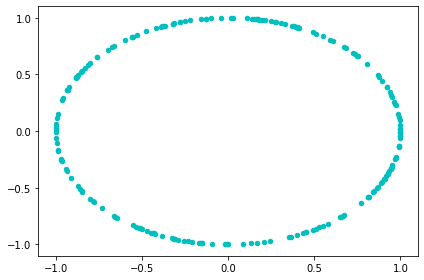
\includegraphics[width=0.4\textwidth]{circle_sampling.png}}
    \subtop[Sphere samples      
    \label{fig:sphere_sampling}]
        {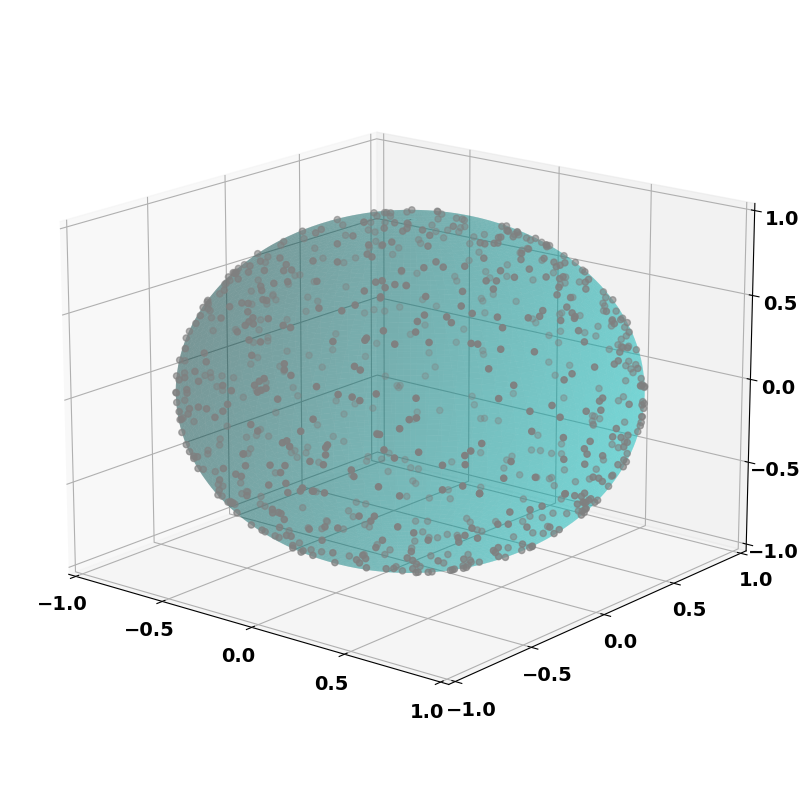
\includegraphics[width=0.4\textwidth]{sphere_sampling.png}}
    \caption{Samples drawn from 1D and 2D manifold.}
\end{figure}

% One popular algorithm for calculating manifolds is diffusion maps \cite{diffusionMaps}, 
% which is a non-linear approach for calculating low-dimensional manifolds
% for (high-dimensional) datasets, using Graph Laplacian.
% Vector diffusion maps \cite{vectorDiffusionMaps} generalize the concept of diffusion maps for vector fields.
% Multi-frequency vector diffusion maps \cite{multiDiffusionMaps} 
% can be seen as an extension to vector diffusion maps, which works well even on highly noisy environments.
% \citet{cryoEmMutliDM} successfully applied multi-frequency vector diffusion Maps in cryo-EM setting,
%  where it was used for denoising purpose.

\subsection{Manifold assumption}
\label{sec:manifoldAssumption}
Manifold assumption is a popular assumption for high-dimensional datasets.
For a given dataset in high-dimension, one can assume that data points are samples drawn from a low-dimensional manifold,
that embeds the high-dimensional space. 
Therefore, if underlying manifold can be approximated, a dimensionality reduction
is established as one can embed data points in the low-dimensional manifold space.
There is a complete area of research devoted to this manifold assumption called Manifold Learning\cite{ManifoldLearning}.

\subsection{Manifold calculation}
\label{sec:manifold_calculation}
Manifold of a dataset can be calculated the following:

\begin{enumerate}
    \item Construct k-NN graph from observations (see section~\ref{sec:graphConstruction}).
    \item Calculate the (normalized) Graph Laplacian.
    \item Extract the second, third (and fourth) smallest eigenvectors.
\end{enumerate}



\subsection{Manifold of computed tomography and cryo-EM}

Therefore, it can be observed how the manifold of classical tomography and cryo-EM objects look like.
In the following, the Shepp-Logan phantom is again used as an example of classical tomography
and the low-dimensional embedding is calculated from the sinogram.



\textbf{TODO: fix figures}
\begin{itemize}
    
    \item TODO: Add perfect circle for k-nn clean sino.
    \item Show that parameter k is important for circle.
    \item Show further that resolution and also sampling pointa matters
    \item Show that with noise, everything gets harder.
    \item Show that exploit the fact that we know the manifold.
\end{itemize}


% In Figure~\ref{fig:phantom_second_third_evec} the manifold calculated from original phantom Graph Laplacian
% can be seen and it is a perfect circle. 
% Further, in figure~\ref{fig:phantom_second_third_evec_noisy}
% noisy version with $\sigma=2$ is plotted and the manifold is not a perfect circle, but circle like.

% The more noise is added, the less manifold looks like a circle. In figure~\ref{fig:phantom_second_third_evec_noisy_high}
% the manifold for $\sigma=100$ is plotted. In all plots, k-NN graphs have been constructed with $k=10$. 


% \begin{figure}[H]
%     \centering
%     \subbottom[Original phantom manifold      \label{fig:phantom_second_third_evec}]{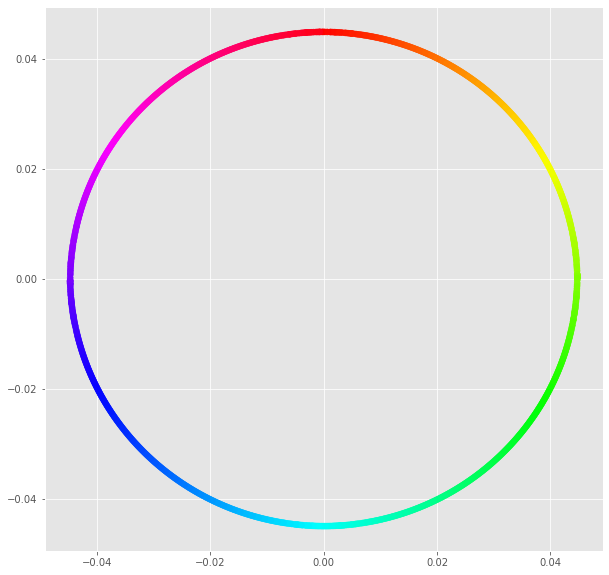
\includegraphics[width=0.25\textwidth]{phantom_second_third_evec.png}}
%     \subbottom[Noisy phantom manifold\label{fig:phantom_second_third_evec_noisy}]{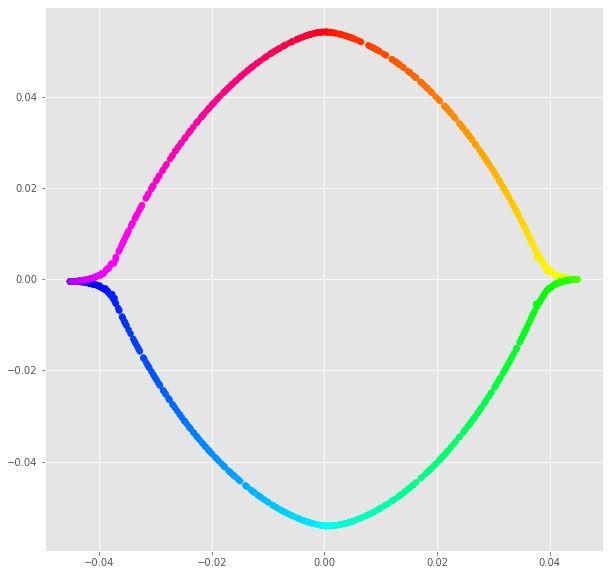
\includegraphics[width=0.25\textwidth]{phantom_second_third_evec_noisy.png}}
%     \subbottom[Highly-noisy phantom manifold \label{fig:phantom_second_third_evec_noisy_high}]{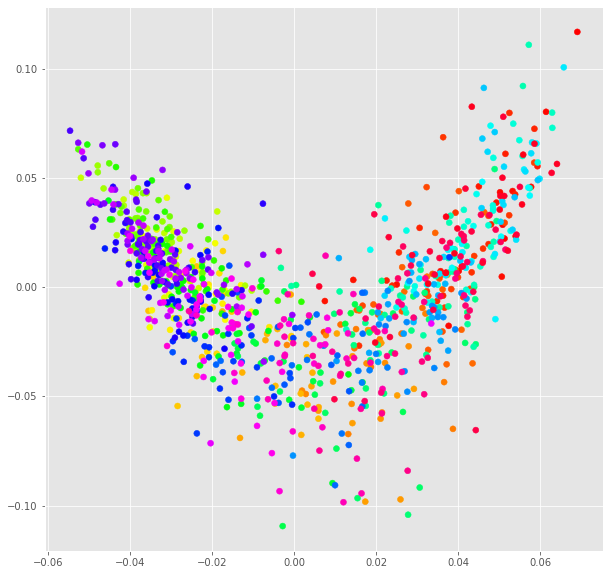
\includegraphics[width=0.25\textwidth]{phantom_second_third_evec_noisy_high.png}}
%     \caption{Shepp-Logan phantom manifolds}
% \end{figure}


\begin{tcolorbox}[colback=red!5!white,colframe=red!75!black]
    In the field of classical tomography and cryo-EM, the underlying low-dimensional manifold is well defined for none-noisy data.
    In the 2D case of classical tomography, the underlying manifold is a circle, whereas in 3D case of cryo-EM the manifold
    is defined as a sphere.
    This fact can be exploited during learning (e.g. by using Wasserstein loss function (see \ref{sec:wasserstein-metric})).
\end{tcolorbox}

\subsection{Connection to Machine Learning}

Graph Laplacian is used for dimensionality reduction for high-dimensional data, as well as spectral clustering and semi-supervised learning.
\citet{LaplaceRandomProjections} used Graph Laplacian in a complete other domain, namely in tomography. 
They showed that Graph Laplacian approximates the Laplace-Beltrami operator.
Further, Graph Laplacian is depended on the adjacency matrix $A$, if $A$ is noisy, Graph Laplacian will be noisy as well.

\section{Graph Deep Learning}
\label{sec:graph_depp_learning}
As already mentioned, Graph Denoising can be seen as a way of link predication. 
The state-of-the-art method for solving link prediction are \textit{Graph Deep Learning} approaches.
Graph Deep Learning is a fast evolving field in research. With Graph Neural Networks (GNN) \cite{GNN} the framework
for neural networks with graphs has been established. 

Using Graph Convolutional Networks (GCN) \cite{GCN} for graph feature extraction is a popular way. 
With GCN a new feature representation is iteratively learned for the node features (edge features are not considered).
It can be seen as an averaging of nodes over their neighbourhood where all neighbours get the same weight combined with some non-linear activation (e.g. ReLU). 
To consider the node itself in averaging they apply the so-called "Renormalization trick", where self-loops are added to the 
adjacency matrix and after every layer, a normalization step is applied. 
The topology of the graph will not be adjusted during  learning process.

\citet{GAT} extended the concept of GCN with attention and not all the neighbouring nodes get the same weight (attention).
Simple Graph Convolutional Network \cite{simpleGCN} proposed a simplified version of GCN.
They could verify their hypothesis that GCN is dominated by local averaging step and non-linear 
activation function between layers do not contribute to much to the success of GCN. 
Therefore, it can be seen as a way of power iteration (see \ref{sec:powerIterations} for further information) over the adjacency matrix with normalization in every layer.
\citet{dynamicGCN} proposed an extension to GCN by not operating on the same graph in every layer but adopting
underlying graph topology layer by layer.

